\documentclass[11pt]{article}
\usepackage[margin=1in]{geometry}
\usepackage[T1]{fontenc}
\usepackage[utf8]{inputenc}
\usepackage{lmodern}
\usepackage{amsmath,amssymb}
\usepackage{booktabs}
\usepackage{graphicx}
\usepackage{siunitx}
\usepackage{physics}
\usepackage{hyperref}
\usepackage[numbers,sort&compress]{natbib}

\hypersetup{
  colorlinks=true,
  linkcolor=blue,
  citecolor=blue,
  urlcolor=blue
}

\sisetup{
  range-phrase=--,
  range-units=single,
  per-mode=symbol
}

\title{Thermalization of Microwave Components in a Dispersive cQED Platform}
\author{Autonomous cQED Research Platform}
\date{April 2, 2026}

\begin{document}
\maketitle

\begin{abstract}
We built a simulation study in \texttt{cqed\_sim} to quantify how a hot microwave component maps onto measurable qubit and cavity observables in a superconducting cQED platform. The study separates four questions: thermometer calibration, thermal-photon-induced dephasing, multimode heating from a hot auxiliary mode, and transient response after a bath-temperature step. The central result is that the cavity occupation is the cleanest thermometer because it tracks the Bose-Einstein occupation nearly one-to-one, while qubit excited-state population is only a secondary, saturating thermometer that requires weak residual dressing beyond the exact dispersive limit. For the representative parameter set used here, thermal loading near \SI{100}{mK} already drives the simulated coherence time below \SI{20}{us}, and a hot auxiliary mode becomes dangerous as soon as it remains appreciably exchange-coupled to the local readout mode. The intrinsic quantum response times are sub-microsecond, so slow variable-temperature-stage traces must originate from macroscopic thermal transport rather than internal cQED equilibration.
\end{abstract}

\section{Introduction}
Thermalization of attenuators, cables, dielectrics, filters, and circulators matters because a cQED device is sensitive not only to nominal stage temperature but also to the effective thermal occupation seen by its electromagnetic modes. In the circuit-QED setting pioneered in Refs.~\cite{blais2004cavity,koch2007transmon}, thermal photons dephase the qubit long before they visibly heat it, and in the strong-dispersive regime those fluctuations can become a dominant coherence limit~\cite{sears2012photon}. The practical question for the present experimental program is therefore not ``what is the cryostat temperature?'' but rather ``what effective occupation and dissipation does the qubit-readout system actually see from a given microwave component?''

This study addresses that question with a deliberately layered model hierarchy implemented in \texttt{cqed\_sim}~\cite{cqed_sim}. The hierarchy matters because the exact dispersive model and the slightly dressed model do not answer the same experimental question. The exact dispersive limit captures cavity thermal occupation and thermal-photon dephasing cleanly, but it cannot heat the qubit population because the qubit number is conserved. A weakly dressed model is therefore required whenever qubit-population thermometry is invoked. Multimode experiments require a further extension in which a hot auxiliary mode can leak into the local readout mode through an exchange channel.

\section{Model Hierarchy and Parameters}
\subsection{Single-mode thermometer and dephasing model}
The baseline transmon-readout Hamiltonian is
\begin{equation}
\frac{H_{\mathrm{disp}}}{\hbar}
=
\omega_q b^\dagger b
+ \frac{\alpha}{2} b^\dagger b^\dagger b b
+ \omega_r a^\dagger a
+ \chi\, a^\dagger a\, b^\dagger b,
\label{eq:h_disp}
\end{equation}
with a thermal readout bath described by
\begin{equation}
\bar n_{\mathrm{th}}(T,\omega_r)=\frac{1}{e^{\hbar \omega_r/(k_B T)}-1}.
\label{eq:nth}
\end{equation}
The Lindblad dissipator is
\begin{equation}
\dot \rho = -\frac{i}{\hbar}[H,\rho]
+ \kappa(\bar n_{\mathrm{th}}+1)\mathcal D[a]\rho
+ \kappa\bar n_{\mathrm{th}}\mathcal D[a^\dagger]\rho
+ \Gamma_1 \mathcal D[b]\rho
+ \Gamma_\phi \mathcal D[n_q]\rho.
\label{eq:lindblad_single}
\end{equation}

To test qubit-population thermometry we also used a weakly dressed model,
\begin{equation}
\frac{H_{\mathrm{dress}}}{\hbar}
=
H_q/\hbar + \omega_r a^\dagger a + g(a^\dagger b + a b^\dagger),
\label{eq:h_dressed}
\end{equation}
which is the minimal extension that lets a hot readout mode admix into the qubit sector. The central point is interpretive: qubit heating is not present in the exact dispersive limit, so any use of qubit population as a thermometer already assumes some residual dressing or leakage channel.

\subsection{Multimode hot-auxiliary model}
The reduced multimode model contains one local readout mode and one hot auxiliary mode,
\begin{equation}
\frac{H_{\mathrm{multi}}}{\hbar}
=
H_q/\hbar
+ \omega_r a_r^\dagger a_r
+ \omega_s a_s^\dagger a_s
+ \chi_r a_r^\dagger a_r\, b^\dagger b
+ \chi_s a_s^\dagger a_s\, b^\dagger b
+ J(a_s^\dagger a_r + a_s a_r^\dagger).
\label{eq:h_multimode}
\end{equation}
The auxiliary mode alone is thermalized; the readout bath and qubit bath are kept cold. A second variant replaces the exact-dispersive qubit-readout coupling with a weak exchange channel so that induced qubit excitation can be estimated as well.

\subsection{Representative parameter set}
Table~\ref{tab:params} summarizes the representative first-pass parameters. These are intended to be cQED-reasonable rather than device-final because the exact project slide values were not available in the current workspace. Whenever a parameter was uncertain, the study promoted it to a sweep axis rather than silently fixing it.

\begin{table}[h]
\centering
\caption{Representative parameters used in the baseline simulations.}
\label{tab:params}
\begin{tabular}{ll}
\toprule
Quantity & Value \\
\midrule
Transmon frequency \(\omega_q/2\pi\) & \SI{5.2}{GHz} \\
Readout frequency \(\omega_r/2\pi\) & \SI{7.0}{GHz} \\
Transmon anharmonicity \(\alpha/2\pi\) & \SI{-220}{MHz} \\
Dispersive shift \(\chi/2\pi\) & \SI{-0.25}{MHz} \\
Weak dressing \(g/2\pi\) & \SI{30}{MHz} \\
Readout decay time \(\kappa_r^{-1}\) & \SI{150}{ns} \\
Intrinsic qubit \(T_1\) & \SI{60}{us} \\
Intrinsic qubit \(T_\phi\) & \SI{120}{us} \\
Multimode hot auxiliary center frequency \(\omega_s/2\pi\) & \SI{7.2}{GHz} \\
Multimode auxiliary linewidth \(\kappa_s^{-1}\) & \SI{120}{ns} \\
\bottomrule
\end{tabular}
\end{table}

\section{Results}
\subsection{A. Thermometer calibration}
Figure~\ref{fig:thermometer} shows the calibration curves. The exact dispersive cavity occupation tracks the target thermal occupation almost exactly from \SI{30}{mK} through \SI{1}{K}, and remains within about \(2\%\) at \SI{2}{K} after the truncation check. Representative values are: \(n_r \approx 1.2\times 10^{-3}\) at \SI{50}{mK}, \(0.036\) at \SI{100}{mK}, \(0.229\) at \SI{200}{mK}, \(1.044\) at \SI{500}{mK}, and \(5.27\) at \SI{2}{K}.

The dressed qubit excited-state population rises strongly at low and intermediate temperature but saturates: \(P_e \approx 1.2\times 10^{-3}\) at \SI{50}{mK}, \(3.35\times 10^{-2}\) at \SI{100}{mK}, \(0.153\) at \SI{200}{mK}, \(0.290\) at \SI{500}{mK}, and \(0.332\) at \SI{2}{K}. The cavity occupation therefore remains the cleanest thermometer, while the qubit population is better viewed as an experimentally convenient alarm channel that signals non-negligible thermal leakage or dressing.

The spectroscopy proxies also become informative in the same regime. The thermally induced linewidth proxy exceeds \SI{0.1}{MHz} near \SI{0.2}{K}, and the simple thermal readout-visibility penalty drops below \(0.9\) near \SI{0.15}{K}. Those two thresholds are especially useful because they connect the microscopic occupation directly to measurements an experimentalist is already likely to perform.

\begin{figure}[t]
\centering
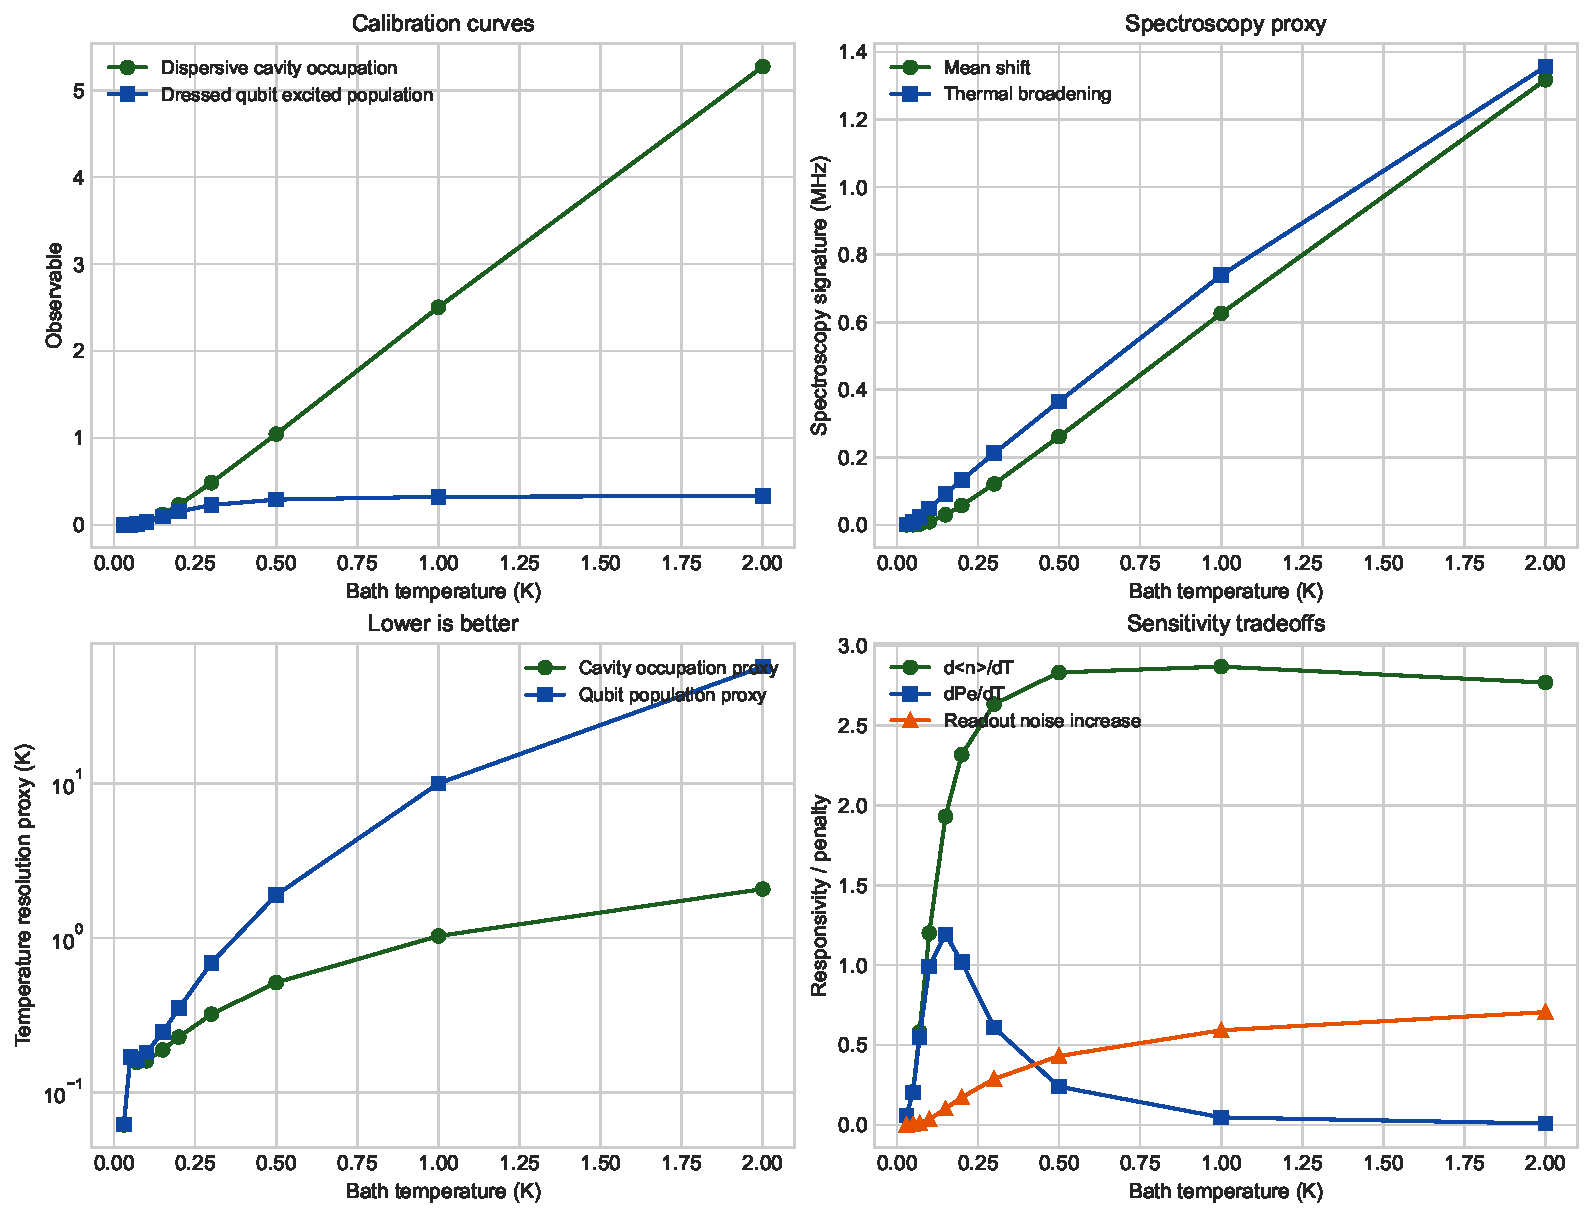
\includegraphics[width=\linewidth]{../figures/thermometer_calibration_curves.pdf}
\caption{Calibration curves for the thermometer study. Top left: exact dispersive cavity occupation and dressed qubit excited-state population versus bath temperature. Top right: thermal spectroscopy shift and broadening proxies. Bottom panels: temperature-resolution proxies and responsivities. The cavity occupation remains the cleanest thermometer across the full sweep because it stays both monotone and nearly linear in the underlying Bose-Einstein occupation.}
\label{fig:thermometer}
\end{figure}

\subsection{B. Thermal-photon-induced dephasing}
Figure~\ref{fig:dephasing} summarizes the coherence study. In the exact dispersive model the Ramsey decay is pure dephasing, as expected. In the weakly dressed model the same hot mode also drives qubit population upward. For the representative parameters, the extracted pure-dephasing rate \(\Gamma_\phi\) rises from roughly \(7.6\times 10^3\,\mathrm{s^{-1}}\) at \SI{30}{mK} to \(1.0\times 10^5\,\mathrm{s^{-1}}\) at \SI{200}{mK} and \(5.2\times 10^5\,\mathrm{s^{-1}}\) at \SI{500}{mK}. The fitted upward heating rate \(\Gamma_\uparrow\) becomes comparable by \SI{100}{mK} and dominates the total coherence budget above about \SI{150}{mK}.

The thermal-limited coherence time falls below the \SI{20}{us} target near \SI{100}{mK}. That is the most important regime-classification result in the study: for the chosen readout linewidth and dispersive shift, \SI{70}{mK} is still tolerable, \SI{100}{mK} is already borderline, and \SI{150}{mK} is clearly dangerous.

The low-occupation analytic estimate
\begin{equation}
\Gamma_{\phi,\mathrm{ana}} \approx \frac{4\chi^2}{\kappa}\bar n_{\mathrm{th}}(\bar n_{\mathrm{th}}+1)
\label{eq:gamma_phi_analytic}
\end{equation}
tracks the numerical trend within a factor of about three over \SI{50}{mK} to \SI{100}{mK}. That is good enough for fast back-of-the-envelope screening, but not good enough to replace the full simulation in the nonlinear regime.

\begin{figure}[t]
\centering
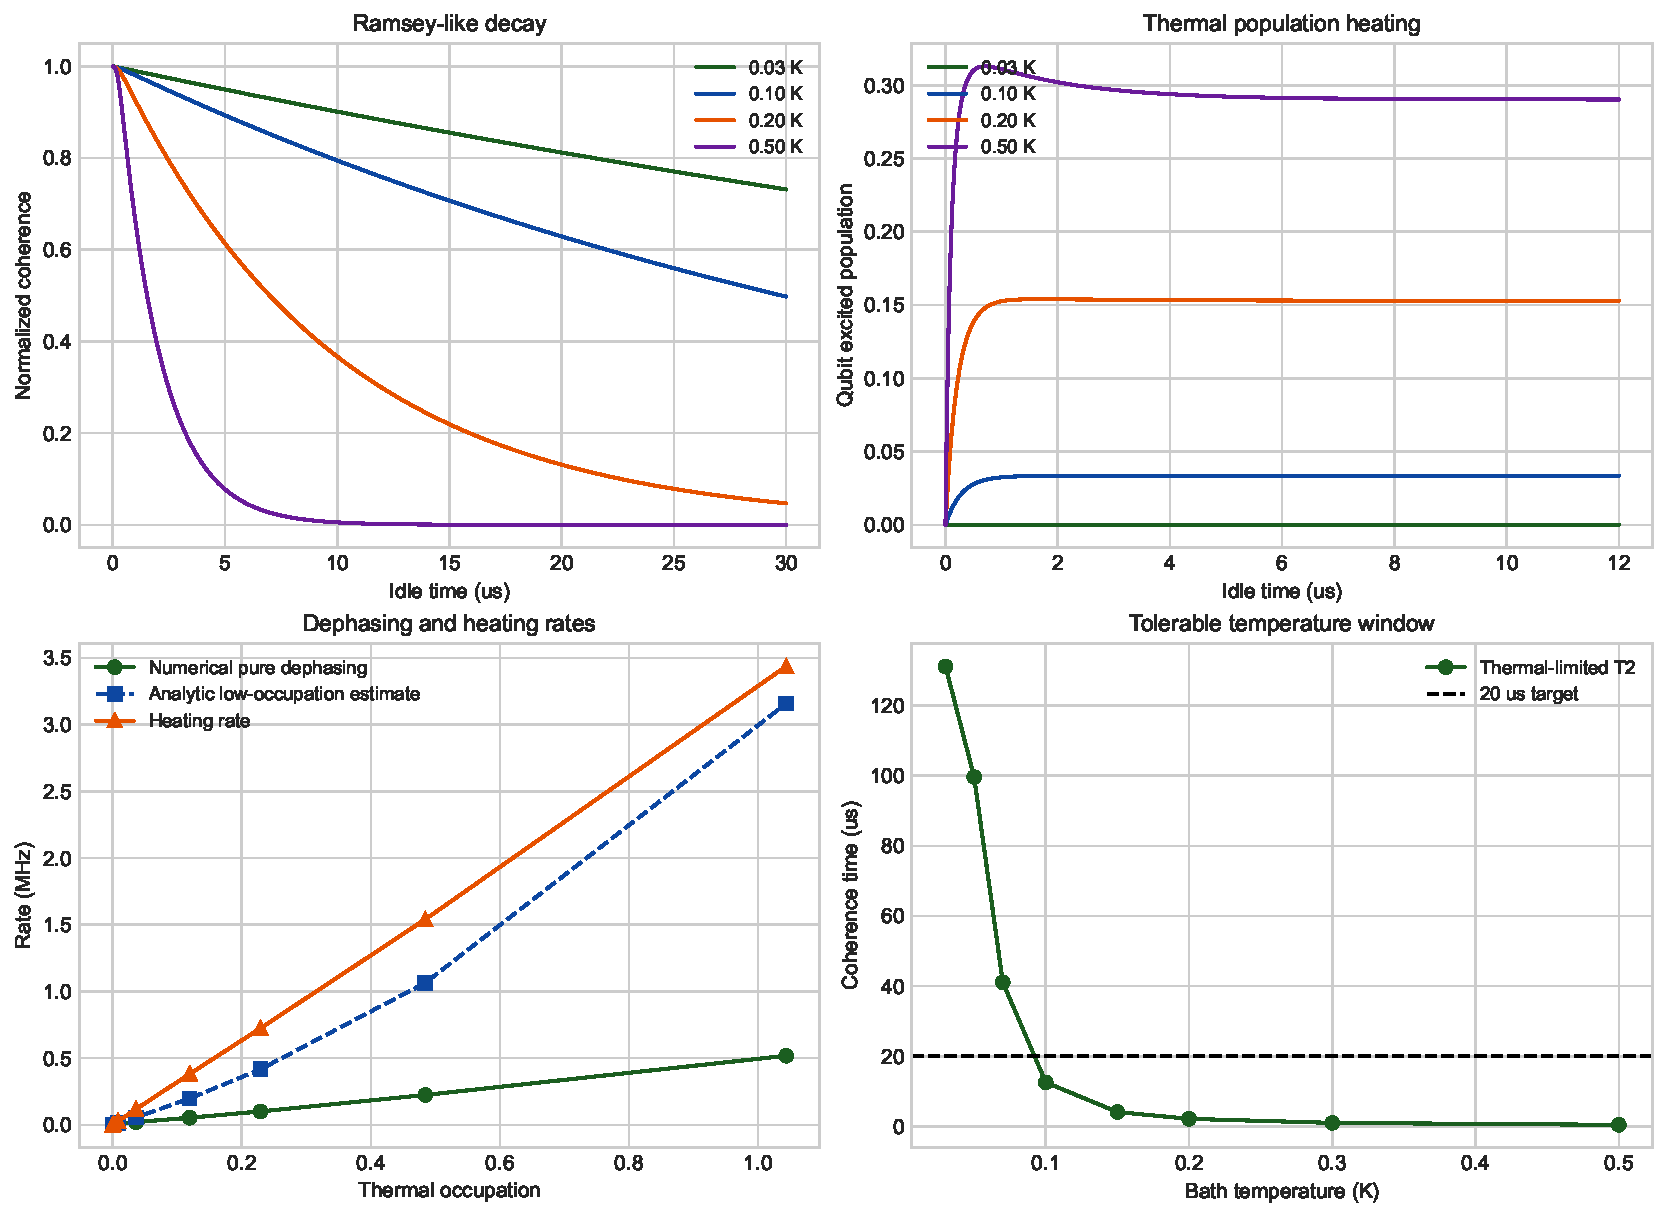
\includegraphics[width=\linewidth]{../figures/dephasing_and_coherence_limits.pdf}
\caption{Thermal dephasing and heating. Top left: representative Ramsey-like coherence traces for several bath temperatures. Top right: dressed-model qubit-heating traces from the ground state. Bottom left: fitted pure-dephasing and heating rates together with the low-occupation analytic estimate. Bottom right: resulting thermal-limited coherence time. The \SI{20}{us} threshold is crossed near \SI{100}{mK}.}
\label{fig:dephasing}
\end{figure}

\subsection{C. Multimode heating and cable-mode leakage}
Figure~\ref{fig:multimode} shows the multimode maps for a hot auxiliary mode coupled to the local readout through an exchange channel \(J\). The safe region is small in this parameter set. Under the joint criterion \(n_r<0.05\), dressed \(P_e<0.01\), and dephasing proxy \(<1/(\SI{20}{us})\), only the \(J=0\) line remained safe.

The main physical lesson is that a hot resonant structure becomes dangerous as soon as it is exchange-coupled strongly enough to leak thermal weight into the readout mode. With \(J/2\pi=\SI{1.5}{MHz}\) the induced readout occupation is already around \(0.3\), and with \(J/2\pi=\SI{12}{MHz}\) the dressed qubit excited-state population reaches \(0.167\) at the most dangerous detuning. Broader hot auxiliary modes are worse rather than better in this reduced model: at fixed \(J/2\pi=\SI{6}{MHz}\) and moderate detuning, reducing the auxiliary lifetime from \SI{300}{ns} to \SI{60}{ns} increases the readout occupation from \(0.220\) to \(0.428\).

\begin{figure}[t]
\centering
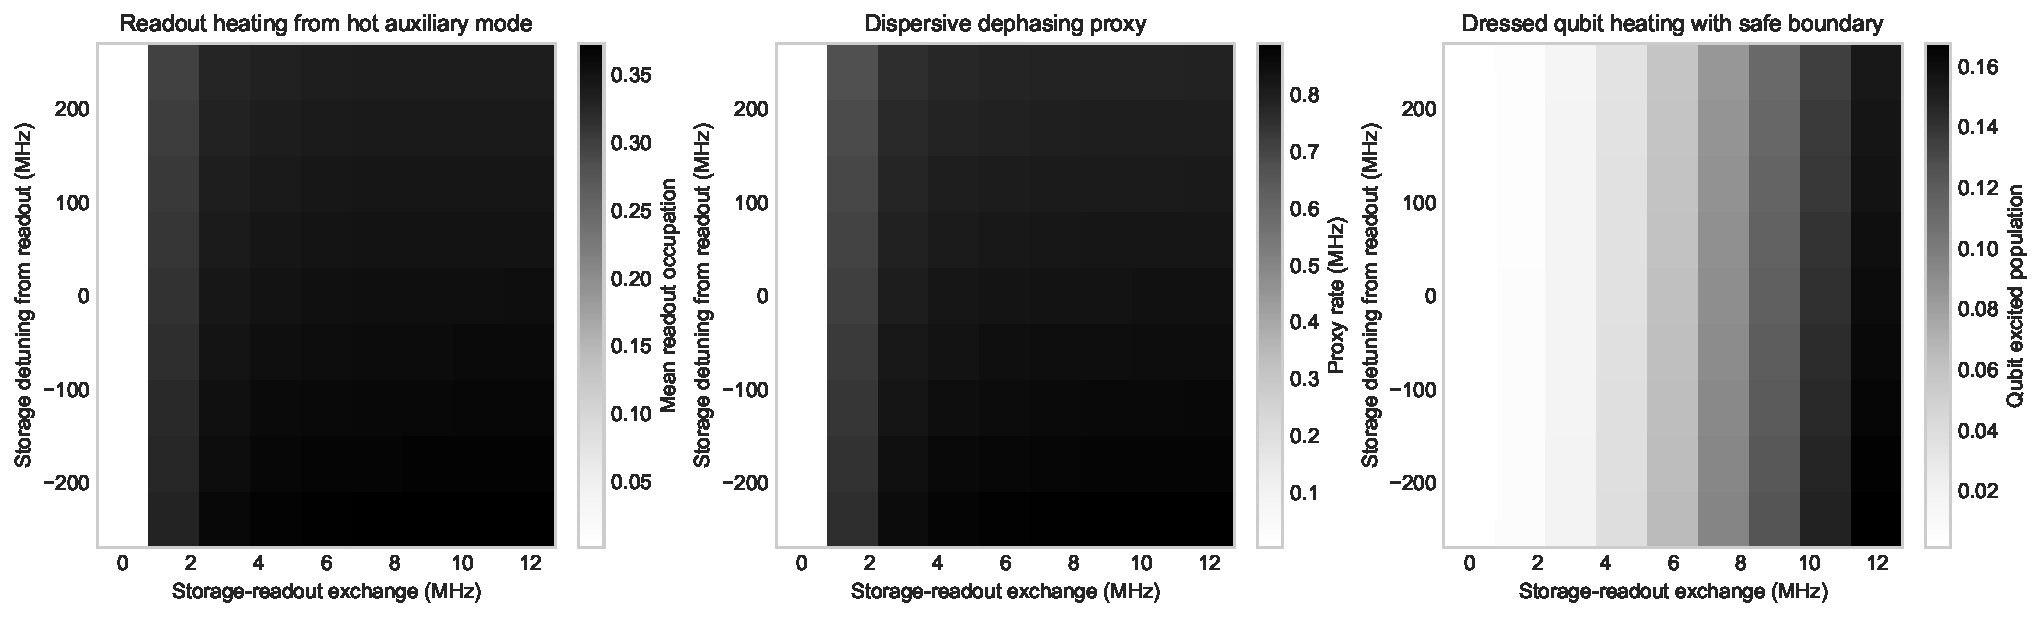
\includegraphics[width=\linewidth]{../figures/multimode_heating_maps.pdf}
\caption{Multimode heating maps for a hot auxiliary mode. Left: induced readout occupation in the exact-dispersive multimode model. Middle: dispersive dephasing proxy extracted from the readout-number variance. Right: dressed qubit excited-state population with a white contour marking the safe-region boundary. In the present parameter set, any appreciable storage-readout exchange is already dangerous if the auxiliary mode is hot.}
\label{fig:multimode}
\end{figure}

\subsection{D. Transient thermal response}
Figure~\ref{fig:transient} shows the intrinsic response after an instantaneous step in bath occupation. The cavity responds with \(\tau \approx \SI{0.15}{us}\) for both steps tested, while the dressed qubit thermometer responds on a similar or faster timescale: \(\SI{0.21}{us}\) for the step to \SI{0.20}{K} and \(\SI{0.089}{us}\) for the step to \SI{0.50}{K}.

This result cleanly separates the quantum and macroscopic problems. The present Lindblad model captures how quickly the cQED subsystem reacts once the effective bath occupation has changed. It does not capture how quickly the component itself heats, cools, or re-equilibrates. Therefore, millisecond-to-second VTS transients should be interpreted as thermal-transport observables and modeled with a separate thermal network that feeds \(n_{\mathrm{th}}(t)\) into the cQED layer.

\begin{figure}[t]
\centering
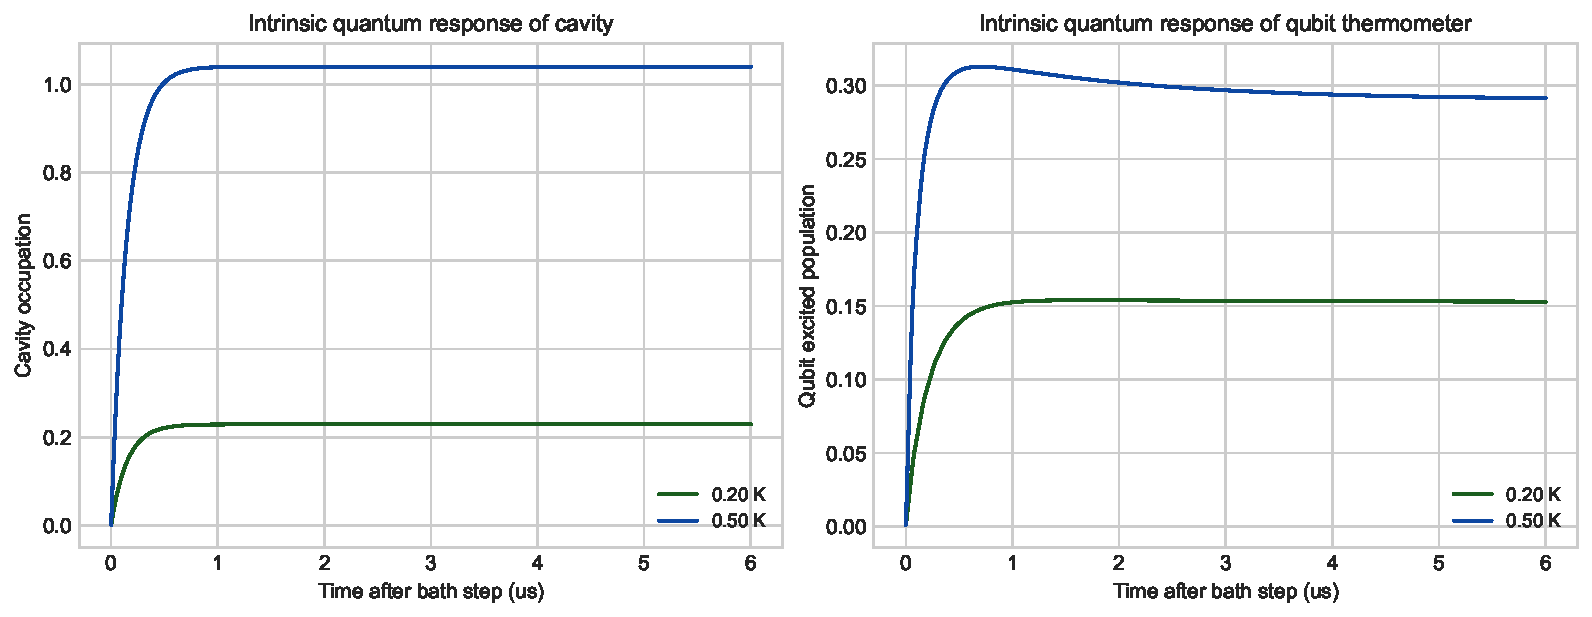
\includegraphics[width=\linewidth]{../figures/transient_thermal_step_response.pdf}
\caption{Intrinsic transient response after an instantaneous bath-temperature step. Left: cavity occupation in the exact dispersive model. Right: qubit excited-state population in the dressed model. The extracted quantum response times are sub-microsecond, which is far faster than any realistic macroscopic thermalization of a cryogenic hardware component.}
\label{fig:transient}
\end{figure}

\section{Validation}
The study passed all targeted validation checks. At zero temperature the cavity occupation and qubit excited-state population both vanished numerically. At \SI{0.20}{K}, the exact dispersive cavity occupation matched the target Bose-Einstein occupation to better than \(10^{-3}\) relative error. The \SI{2}{K} thermometer point changed by only about \(2.0\%\) when the cavity truncation was increased from 30 to 36 photons. The fitted dephasing rate at \SI{0.20}{K} changed by less than \(10^{-6}\) relative when the dynamic truncation was increased from 12 to 14 photons. In the multimode study, the weak-coupling limit returned the readout to its cold-bath occupation, and representative truncation checks changed the readout occupation and dressed qubit excitation by less than \(3\%\).

\section{Experimental Guidance}
The simulations support five direct recommendations.

\begin{enumerate}
\item Measure cavity-occupation or spectroscopy-broadening proxies first. They are the closest observables to the true thermal occupation.
\item Use qubit excited-state population as a secondary alarm channel rather than the primary calibrated thermometer. It is more nonlinear and saturates strongly.
\item Treat \SI{100}{mK} effective mode temperature as a warning threshold for the present parameter set, because the thermal-limited coherence already falls below \SI{20}{us}.
\item In multimode experiments, prioritize detuning and exchange suppression before attempting precision thermometry. A hot auxiliary mode that remains appreciably coupled is already a dominant error channel.
\item Interpret slow VTS transients as thermal-transport data. The internal cQED subsystem equilibrates on sub-microsecond timescales in the present model.
\end{enumerate}

\section{Limitations and Future Work}
The study does not model boundary resistance, distributed cable temperature profiles, dielectric relaxation, or non-Markovian thermal noise. The hot component appears only through an effective bath occupation or a hot auxiliary mode. Exact SNAILmon-cable slide parameters were unavailable in the workspace, so the multimode numbers should be read as regime-defining rather than device-final.

The most realistic next step is to couple this cQED layer to a separate thermal model. A lumped thermal RC model, or a more detailed finite-element thermal calculation, can provide the time-dependent effective temperature of the relevant component or electromagnetic mode. That \(T(t)\) can then be converted to \(\bar n_{\mathrm{th}}(t)\) through Eq.~\eqref{eq:nth} and fed into the present quantum model to predict qubit excitation, dephasing, and readout degradation.

\section{Reproducibility}
The study includes machine-readable artifacts for each thrust and an executable notebook that reproduces the main figures from a single parameter cell. The numerical workflow uses the public \texttt{cqed\_sim} dispersive and multimode models wherever available; the only documented local bridge is the steady-state helper, which keeps the \texttt{cqed\_sim} Hamiltonian and Lindblad conventions intact while calling QuTiP's steady-state solver because the public package does not yet expose a dedicated steady-state entry point.

\appendix
\section{Detailed Results and Data}
\subsection{Representative thermometer points}
At \SI{50}{mK}, the simulated cavity occupation is \(1.2\times 10^{-3}\) and the dressed qubit excited-state population is \(1.2\times 10^{-3}\). At \SI{100}{mK}, those values are \(0.036\) and \(0.0335\), respectively. At \SI{200}{mK}, the cavity occupation is \(0.229\), the dressed qubit excited-state population is \(0.153\), the spectroscopy broadening proxy is \SI{0.133}{MHz}, and the readout-visibility penalty has already fallen to approximately \(0.83\).

\subsection{Representative coherence points}
The thermal-limited coherence times extracted from the combined dephasing-plus-heating model are approximately \SI{131}{us} at \SI{30}{mK}, \SI{100}{us} at \SI{50}{mK}, \SI{41}{us} at \SI{70}{mK}, \SI{12.5}{us} at \SI{100}{mK}, \SI{4.10}{us} at \SI{150}{mK}, \SI{2.16}{us} at \SI{200}{mK}, \SI{1.01}{us} at \SI{300}{mK}, and \SI{0.45}{us} at \SI{500}{mK}.

\subsection{Representative multimode points}
With a hot auxiliary mode at \SI{350}{mK}, the weak-coupling limit \(J=0\) returns the readout to its cold-bath occupation. At moderate exchange, the local readout occupation climbs to roughly \(0.30\) to \(0.37\) across the detuning range. The dressed qubit excitation peaks at \(0.167\) for the most dangerous point in the scanned grid, corresponding to large exchange and the largest negative detuning tested.

\bibliographystyle{unsrtnat}
\bibliography{references}

\end{document}
